\documentclass[a4paper,12pt]{article}
\usepackage[margin=1in]{geometry}

\usepackage[T2A]{fontenc}			% кодировка
\usepackage[utf8]{inputenc}			% кодировка исходного текста
\usepackage[english,russian]{babel}	% локализация и переносы
\usepackage{graphicx}                % Математика
\usepackage{amsmath,amsfonts,amssymb,amsthm,mathtools} 
\usepackage{mathtext}
\usepackage[T2A]{fontenc}
\usepackage[utf8]{inputenc}

\usepackage{wasysym}

%Заговолок
\author{Бичина Марина 
группа Б04-005 1 курса ФЭФМ}
\title{}
\date{}


\begin{document} % начало документа

\begin{center}
\begin{Large}
{Бичина Марина Б04-005, Лабораторная работа №. 6.9.1 <<закон Кюри-Вейсса и обменное взаимодействие в ферромагнетиках>>}
\end{Large}
\end{center}
\paragraph{Цель работы:} 
\begin{enumerate}
\itemsep0em
\item Исследовать температурную зависимость магнитной восприимчивости ферромагнетика в парамагнитной области -- выше точки Кюри
\item По полученной температуре Кюри оценить энергию обменного взаимодействия
\end{enumerate}

\paragraph{Теоретическая справка:}
Намагниченность вещества $I$ связана с внешним магнитным полем $H$, под воздействием которого она возникает, соотношением 
\[
I = \varkappa H,
\]
где $\varkappa$ называется магнитной восприимчивостью. Рассмотрим, чем определяется восприимчивость парамагнитного вещества, в котором магнитный момент атома обусловлен спином одного электрона. Магнитный момент электрона $\boldsymbol{\mu}$ во внешнем поле будет направлен либо по, либо против поля, поэтому в магнитном поле возникнут энергии
\[
E_{\pm} = \pm\mu B,
\]
причём в состоянии $E_-$ магнитный момент параллелен полю. Отношения числа частиц на этих уровнях
\[
\dfrac{N_+}{N_-} = \exp\left(- \dfrac{2\mu B}{k_{\text{Б}}T} \right) \approx 1 - \dfrac{2\mu B}{k_{\text{Б}}T},
\]
здесь приближение оправдано, так как даже для $B = 10^5~\text{Гс}$ при $T = 300~\text{К}$ будет справедливо $2\mu B/k_{\text{Б}}T \approx 0.05$, а значит, мы можем считать $\mu B \ll k_{\text{Б}}T$. Соответственно, намагниченность определяется разностью чисел электроннов на двух уровнях
\[
\Delta N = N_- - N_+ \approx N \dfrac{\mu B}{k_{\text{Б}}T},
\]
где $N = N_- + N_+$ -- количество неспаренных электронов в единице объёма. Отсюда, учётывая $I = \mu \Delta N$ и $H \approx B$, получаем
\begin{equation}\label{1}
\varkappa = \dfrac{I}{H} = N\dfrac{\mu^2}{k_{\text{Б}}T}.
\end{equation}
Для атома с более чем одним электроном и суммарным спином $S$, эта формула обобщается как
\[
\varkappa = \dfrac{Ng^2 \mu_{\text{Б}}^2S(S+1)}{3k_{\text{Б}}T}
\]
где $g$ -- фактор Ланде.\\
В ферромагнетиках для описание взаимодействия соседних электронов вводится эффективное (или обменное) поле $H_{\text{эфф}}$, величина которого пропорциональна намагниченности:
\[
H_{\text{эфф}} = \lambda I,
\]
где $\lambda$ -- некоторая константа. С учётом этого поля формула (\ref{1}) перепишется как
\[
\varkappa = \dfrac{I}{H} = N\dfrac{g^2 \mu_{\text{Б}}^2 S(S+1)}{3k_{\text{Б}}(T-\Theta)},
\]
где 

\begin{equation}
\varkappa \propto \dfrac{1}{T - \Theta}
\end{equation}
называемое \textbf{\textit{законом Кюри--Вейса}}. Температура $\Theta$ называется парамагнитной точкой Кюри, при стремлении температуры к ней восприимчивость неограниченно возрастает из-за того, что тепловое движение всё меньше препятствует магнитным моментам ориентироваться в одном направлении. \textit{Это не то же самое, что точка Кюри $T_\text{C}$, которая определяется как температура фазового перехода из парамагнитного в ферромагнитное состояние. Как правило, $\Theta > T_\text{С}$.}\\
Теперь выясним связь обменного интеграла с $\Theta$. Исходя из наличия эффективного поля $H_{\text{эфф}}$, получаем, что энергия, которую необходимо затратить на то, чтобы перевернуть один спин, может быть получена как 
\begin{equation}\label{2}
U_{\text{пер}} = 2\mu H_{\text{эфф}} = 2 \mu \cdot \lambda I = 2\mu \dfrac{\lambda \mu}{V},
\end{equation}
где $V$ -- объём, приходящийся на один атом. В то же время, эта энергия переворота в два раза больше обменной энергии системы, так как можно показать, что энергии систем с параллельными и антипаралалльными спинами отличаются знаком. Обменная энергия равна 
\[
U_{\text{обм}} = -2J \mathbf{S}_i \mathbf{S}_j,
\]
 где $J$ -- обменный интеграл, $\mathbf{S}_i \mathbf{S}_j$ скалярное произведение векторов спинов, поэтому в итоге
\[
U_{\text{пер}} = 2 (2JnS^2),
\]
где $S$ -- среднее значение $\mathbf{S}$ вдоль направления намагниченности, $n$ -- число соседей. Таким образом, с учётом (\ref{2}) и $\mu = gS\mu_\text{Б}$, получаем
\[
\lambda = \dfrac{2nJV}{g^2\mu^2_\text{Б}}.
\]
Учитывая, что $V = 1/N$, где $N$ -- концентрация атомов, то, с учётом определения $\Theta$ получим окончательно
\begin{equation}\label{4}
J = \dfrac{3k_\text{Б}\Theta}{2nS(S+1)}
\end{equation}

\paragraph{Описание установки:}
\begin{figure}[h]
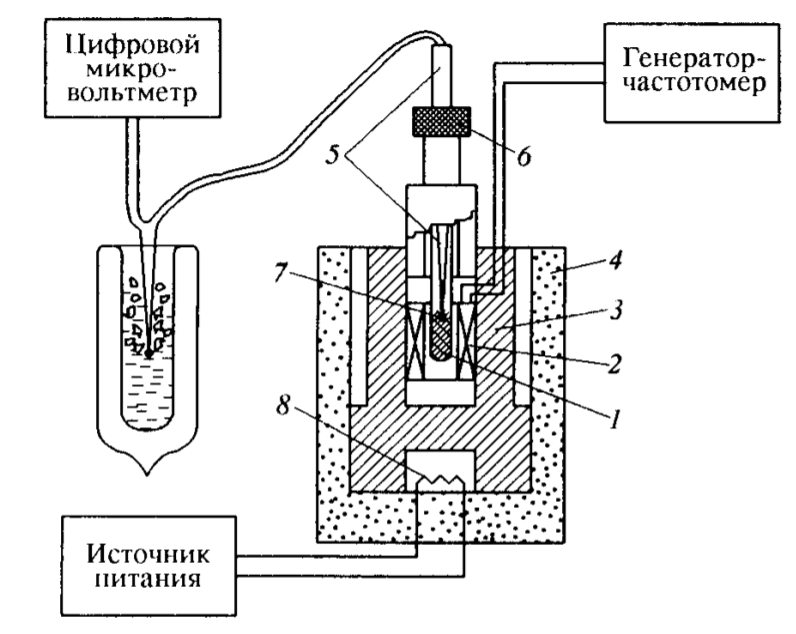
\includegraphics[width = 0.55\textwidth]{1.png}
\centering
\caption{Схема экспериментальной установки.}
\end{figure}

Ферромагнитный образец 1 располагается внутри пустотелой катушки 2, которая является индуктивностью колебательного контура, входящего в состав LC-генератора.\\ Катушка самоиндукции помещена в термостат, представляющий собой массивный медный цилиндр 3, расположенный в пенопластовом корпусе 4. С помощью термостата производится охлаждение образца.\\ Исследуемый ферромагнетик (в нашей работе это гадолиний Gd) является проводником, а рабочая частота генератора высока, поэтому для того, чтобы не возникло токов Фуко, образец изготовлен из мелких гранул размером менее 0.1 мм. Он помещён в тефлоновую капсулу, которую с помощью штока 5 можно перемещать вдоль катушки самоиндукции.\\

Магнитная восприимчивость образца определяется по изменению самоиндукции при его введению в катушку:\\ Пусть $L$ -- индуктивность с образцом, а $L_0$ -- без \\ Тогда
\[
L = \mu L_0,
\]
где $\mu$ -- магнитная проницаемость образца, т.е.
\[
\dfrac{L - L_0}{L_0} = \dfrac{\Delta L}{L_0} = \mu - 1.
\]
Принимая в расчёт, что длина образца сильно больше его диаметра, можно пренебречь размагничивыющим фактором, тогда
\[
\dfrac{L - L_0}{L_0} = \dfrac{\Delta L}{L_0} = \mu - 1 = 4\pi \varkappa.
\]
С учётом того, что собственная частота контура обратно пропорциональна корню из индуктивности, получим
\begin{equation}\label{5}
\dfrac{1}{\varkappa} \propto \dfrac{f^2}{f_0^2 - f^2}
\end{equation}

Для рабочей установки:\\
1. Истинный 0: 0.03 мВ \\
2. Константа термопары: 41 мкВ/К\\
3. Комнатная температура: 24 $^oC$
\paragraph{Ход работы:}
\begin{enumerate}
\itemsep0em
\item Произведем измерения в интервале температур от 274 К до 320 К Охлаждение образца производится с помощью массивного медного цилиндра 3, который предварительно охлаждается в морозильнике бытового холодильника или при помощи жидкого азота \\ Для нагревания служит электронагреватель 8, находящийся в тепловом контакте с
цилиндром 3\\ Данные, полученные в ходе эксперимента, приведены в таблице 1
\begin{table}[h!]
\centering
\begin{tabular}{|l|l|l|l|l|l|l|l|l|}
\hline
U, мВ & T, K    & f, кГц  & $f_0$, кГц &  & U, мВ & T, K    & f, кГц & $f_0$, кГц \\ \hline
-0.9  & 274.317 & 803.885 & 857.049    &  & 0.14  & 299.683 & 851.3  & 858.149    \\ \hline
-0.82 & 276.268 & 803.833 & 856.99     &  & 0.27  & 302.854 & 852.78 & 858.35     \\ \hline
-0.72 & 278.707 & 803.796 & 857.081    &  & 0.40  & 306.024 & 853.97 & 858.41     \\ \hline
-0.59 & 281.878 & 804.358 & 857.081    &  & 0.51  & 308.707 & 854.5  & 858.41     \\ \hline
-0.46 & 285.049 & 805.577 & 857.289    &  & 0.61  & 311.146 & 854.99 & 858.58     \\ \hline
-0.33 & 288.220 & 811.200 & 857.405    &  & 0.71  & 313.585 & 855.4  & 858.616    \\ \hline
-0.23 & 290.659 & 820.875 & 857.615    &  & 0.81  & 316.024 & 855.84 & 858.630    \\ \hline
-0.11 & 293.585 & 837.475 & 857.921    &  & 0.91  & 318.463 & 856.08 & 858.85     \\ \hline
0.02  & 296.756 & 847     & 858.147    &  & 1.01  & 320.902 & 856.27 & 858.801    \\ \hline
\end{tabular}
\caption{Зависимость частот от температуры образца}
\end{table}
\item По данным из таблицы построим график зависимости $\dfrac{f^2}{f^2_0-f^2}(T)$ по МНК на участке, где зависимость будет линейно-возрастающей: \\
Для нашей работы зависимость будет выглядеть как \\$y = (5.39 \pm 0.12)x - 1559 \pm 38$ (y = kx + b, $k=5.39 \pm 0.12$, $b=-1559 \pm 38$)
\begin{figure}[h!]
\includegraphics[scale=0.8]{../../../../Users/Marina/вычматы/Untitled Folder/plot_9_1.pdf} 
\end{figure}
\item Вычислим точку Кюри для ферромагнетика, исходя из условия $y=0$
\[(5.39 \pm 0.12)\theta - 1559 \pm 38 = 0\]
\[\theta = \frac{1559}{5.39} \approx 289 K \]
Погрешность можно найти по формуле 
\[
\Delta \Theta = \Theta \sqrt{\left( \frac{\Delta k}{k} \right)^2 + \left( \frac{\Delta b}{b} \right)^2} = 289 \sqrt{\left( \frac{0.12}{5.39} \right)^2 + \left( \frac{38}{1559} \right)^2} = 9 \text{ К},
\]
Окончательно получим 
\begin{equation}
\theta = 290 \pm 9\;\; K
\end{equation}
\item Оценим величину обменного интеграла J (примем для гадолиния $n=12\;\; S=7/2$) по формуле \ref{4}
\[J=\frac{3k_{\text{Б}}\cdot 290}{2\cdot12\cdot3,5\cdot4,5} \approx 3.18\cdot 10^{-16}\;\;\text{эрг} = 198\;\;\text{мкэВ}\]
Погрешность:
\[\Delta J = J\frac{\Delta\theta}{\theta} = 6\;\;\text{мкэВ}\]
Окончательно получим: 
\begin{equation}
J = 200 \pm 6\;\;\text{мкэВ}
\end{equation}
\end{enumerate}
\paragraph{Выводы:}
\begin{enumerate}
\item В ходе работы была исследована температурная зависимость магнитной восприимчивости гадолиния и определена температура Кюри $\Theta = 290 \pm 9~\text{К}$
\item По полученному значению $\Theta$ был оценен обменный интеграл $J = 200\pm 6~\text{мкэВ}$.

\end{enumerate}
\end{document}